% =====================================================================
% SUPPLEMENTARY NOTE 2 — the scIB scorecard on this corpus.
%
% SOURCES. Every number is read from Outputs/supplementary/scib/, which
% figures/scripts/scib_table.py builds from the auditors' own manifest by
% exact key (method, gene policy, fit split). The tables below are
% generated fragments in ../tables/; nothing is typed.
%
% THE FAIRNESS CONSTRAINT, settled 11 November: Hrovatin's authors wrote
% scIB. The claim is that its axes do not discriminate ON THIS CORPUS,
% never that the framework is wrong. Every paragraph here is written to
% that line.
% =====================================================================

\section{The scIB scorecard on this corpus}
\label{note:scib}

The main text measures batch removal and biological conservation with two
instruments built for this corpus, donor recovery and cross-donor agreement
(Methods, \emph{Cross-donor agreement}). The field's standard instrument is
the scIB battery \citep{luecken2022benchmarking}, ten metrics in two halves,
and the atlas-building review recommends it for choosing an integration
\citep{hrovatin2025atlases}. Every representation in Table~1 was therefore
scored on all ten. This note reports the full scorecard, says which of the
ten discriminate between representations here, and explains why the ones
that do are ranking on something other than the quantity the paper is
about. The claim throughout is about this corpus. scIB was built to rank
integrations of multi-dataset atlases where the batch is the dataset and the
biology to conserve is cell type; on such atlases it does what it was built
for, and nothing below says otherwise.

\subsection{What was scored}

Ten metrics were computed with the scib-metrics implementation on the
176{,}803 held-out cells that carry a cell-family label, which come from the
two studies that annotated their own cells. The batch variable is study and
the label has four levels. Seven of the ten were also computed against the
sixty-level \texttt{AnnotationRefined} vocabulary over 132{,}261 cells; that
vocabulary comes from one study, so the three metrics that compare studies
within a label have no second study to compare and are not defined on it.
Eleven representations were scored: the two reported \elaj{} arms, five
integration and dimension-reduction methods and four pretrained foundation
models, each on the cells and gene policy recorded in the auditors'
manifest. One cell of the table has a different provenance and it is
declared: scFoundation's silhouette-batch score comes from a re-scoring pass
over the same dumped latent, because the first pass was killed inside that
metric; the re-scoring reproduced all seven metrics it shares with the first
pass to the printed precision, which is what makes the one new value usable.
Table~\ref{stab:scib-family} is the scorecard on cell family and
Table~\ref{stab:scib-refined} the one on the finer vocabulary.
Supplementary Fig.~\ref{sfig:scib-heatmap} draws the first.

\begin{table}[p]
\centering
\caption[scIB scorecard, cell family]{\textbf{The scIB scorecard on cell
family.} Eleven representations, ten metrics, 176{,}803 held-out cells
from the two studies that annotated their cells; batch is study. The five
columns on the left are scIB's batch-correction half and the five on the
right its biological-conservation half. Every metric is scaled so that one
is best.}
\label{stab:scib-family}
\footnotesize\setlength{\tabcolsep}{3pt}
\resizebox{\textwidth}{!}{% GENERATED by figures/scripts/supp_figures.py. Do not edit by hand.
\begin{tabular}{@{}lrrrrrrrrrr@{}}
\toprule
representation & graph conn. & iLISI & kBET & PCR batch & silhouette batch & ARI & cLISI & isolated labels & NMI & silhouette bio \\
\midrule
\elaj\,B\textsubscript{hi} & 0.9854 & 0.0000 & 0.0051 & 0.8603 & 0.7727 & 0.0498 & 1.0000 & 0.6066 & 0.0724 & 0.6157 \\
\elaj\,B\textsubscript{lo} & 0.9851 & 0.0000 & 0.0400 & 0.8295 & 0.7176 & 0.1708 & 1.0000 & 0.5991 & 0.3364 & 0.5824 \\
\midrule
PCA & 0.7232 & 0.0000 & 0.0000 & 0.5249 & 0.4649 & 0.2026 & 1.0000 & 0.6098 & 0.2576 & 0.6206 \\
scVI & 0.9855 & 0.0000 & 0.0150 & 0.9268 & 0.8554 & 0.3495 & 1.0000 & 0.6055 & 0.4417 & 0.6157 \\
scANVI & 0.9832 & 0.0000 & 0.0210 & 0.9386 & 0.8656 & 0.3390 & 1.0000 & 0.6230 & 0.4473 & 0.6272 \\
Harmony & 0.9724 & 0.0000 & 0.0400 & 0.8341 & 0.8464 & 0.2821 & 1.0000 & 0.6115 & 0.4046 & 0.5910 \\
Scanorama & 0.7116 & 0.0000 & 0.0001 & 0.5149 & 0.5178 & 0.1980 & 1.0000 & 0.5738 & 0.2397 & 0.5835 \\
\midrule
scGPT & 0.9685 & 0.0000 & 0.0184 & 0.9091 & 0.8909 & 0.4205 & 1.0000 & 0.6592 & 0.5735 & 0.6806 \\
Geneformer & 0.9577 & 0.0000 & 0.0001 & 0.7607 & 0.7197 & 0.0766 & 1.0000 & 0.5145 & 0.0651 & 0.5363 \\
SCimilarity & 0.8825 & 0.0000 & 0.0007 & 0.8181 & 0.7150 & 0.9010 & 1.0000 & 0.7483 & 0.8555 & 0.8060 \\
scFoundation & 0.8051 & 0.0000 & 0.0013 & 0.7689 & 0.7540 & 0.2332 & 1.0000 & 0.6681 & 0.3447 & 0.6918 \\
\bottomrule
\end{tabular}
}
\end{table}

\begin{table}[p]
\centering
\caption[scIB scorecard, refined annotation]{\textbf{The scIB scorecard on
the sixty-level annotation.} The seven metrics that are defined when the
label comes from a single study, over 132{,}261 held-out cells carrying
\texttt{duempelmann\_2026}'s \texttt{AnnotationRefined}. PCR batch is one
for every representation because there is one study, so the variance
explained by study is zero before and after.}
\label{stab:scib-refined}
\small
% GENERATED by figures/scripts/supp_figures.py. Do not edit by hand.
\begin{tabular}{@{}lrrrrrrr@{}}
\toprule
representation & graph conn. & PCR batch & ARI & cLISI & isolated labels & NMI & silhouette bio \\
\midrule
\elaj\,B\textsubscript{hi} & 0.4480 & 1.0000 & 0.0306 & 0.9977 & 0.4658 & 0.3152 & 0.4589 \\
\elaj\,B\textsubscript{lo} & 0.3649 & 1.0000 & 0.0258 & 0.9968 & 0.4358 & 0.2726 & 0.4354 \\
\midrule
PCA & 0.5006 & 1.0000 & 0.0358 & 0.9977 & 0.4622 & 0.3192 & 0.4478 \\
scVI & 0.5717 & 1.0000 & 0.0284 & 0.9980 & 0.4927 & 0.3199 & 0.4702 \\
scANVI & 0.5934 & 1.0000 & 0.0287 & 0.9981 & 0.4932 & 0.3234 & 0.4712 \\
Harmony & 0.4852 & 1.0000 & 0.0288 & 0.9984 & 0.4759 & 0.3129 & 0.4458 \\
Scanorama & 0.5340 & 1.0000 & 0.0323 & 0.9984 & 0.4877 & 0.3275 & 0.4689 \\
\midrule
scGPT & 0.4931 & 1.0000 & 0.0281 & 0.9973 & 0.4912 & 0.3008 & 0.4764 \\
Geneformer & 0.3189 & 1.0000 & 0.0176 & 0.9963 & 0.4492 & 0.1854 & 0.4430 \\
SCimilarity & 0.5683 & 1.0000 & 0.0460 & 0.9981 & 0.4991 & 0.3532 & 0.4842 \\
scFoundation & 0.5648 & 1.0000 & 0.0336 & 0.9983 & 0.6071 & 0.3272 & 0.6362 \\
\bottomrule
\end{tabular}

\end{table}

\begin{figure}[p]
\centering
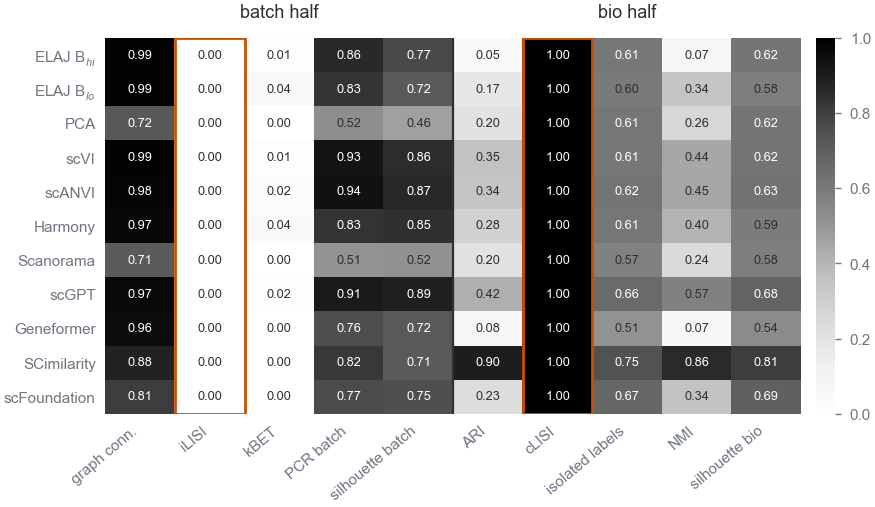
\includegraphics[width=.95\textwidth]{figures/scib_scorecard_heatmap.png}
\caption[The scorecard as a heatmap]{\textbf{Table~\ref{stab:scib-family}
drawn.} Darker is better on every metric. The two outlined columns, iLISI
and cLISI, take one value for all eleven representations.}
\label{sfig:scib-heatmap}
\end{figure}

\subsection{Two of the ten are constants here, and a third nearly}

iLISI is 0.0000 for all eleven representations and cLISI is 1.0000 for all
eleven. kBET spans 0.0000 to 0.0400. Representations that differ by 0.27 in
donor recovery, by 0.30 in cross-donor cycle agreement and by 0.19 in study
separation receive identical scores from two of the ten metrics, so neither
can rank them, whatever the reason (Table~\ref{stab:scib-disc},
Supplementary Fig.~\ref{sfig:scib-range}). The reason is structural rather
than numerical. Both LISI scores are medians, over cells, of the effective
number of categories in a cell's neighbourhood. The labelled cells come from
two studies at a three-to-one imbalance, 132{,}259 against 44{,}544, and in
every representation the typical labelled neighbourhood draws on one study
and one family. The first puts iLISI at its floor; the second puts cLISI at
its ceiling, and it is the same fact the main text reports as cell family
being saturated across the field, 0.9023 to 0.9896 cross-donor. kBET asks a
stricter form of the iLISI question, whether the local study mix matches the
global one, and 0.04 is the most any representation achieves.

\begin{table}[t]
\centering
\caption[What each scIB metric discriminates here]{\textbf{Range of each
metric across the eleven representations.} A metric whose range is below
the rounding the paper reports cannot rank representations on this corpus.
The description of what each metric rewards is a one-clause reading of its
definition in \citet{luecken2022benchmarking}.}
\label{stab:scib-disc}
\footnotesize
% GENERATED by figures/scripts/supp_figures.py. Do not edit by hand.
\begin{tabular}{@{}llp{52mm}rrrl@{}}
\toprule
metric & half & rewards & min & max & range & on this corpus \\
\midrule
graph conn. & batch & each label's cells form one connected kNN component & 0.7116 & 0.9855 & 0.2739 & discriminates \\
iLISI & batch & neighbourhoods draw on many studies & 0.0000 & 0.0000 & 0.0000 & constant \\
kBET & batch & local study mix matches the global mix & 0.0000 & 0.0400 & 0.0400 & near-constant \\
PCR batch & batch & variance explained by study after, against before & 0.5149 & 0.9386 & 0.4237 & discriminates \\
silhouette batch & batch & within a label, studies do not separate & 0.4649 & 0.8909 & 0.4260 & discriminates \\
\midrule
ARI & bio & Leiden clusters coincide with the label & 0.0498 & 0.9010 & 0.8512 & discriminates \\
cLISI & bio & neighbourhoods draw on one label & 1.0000 & 1.0000 & 0.0000 & constant \\
isolated labels & bio & the rarest-across-studies label stays separable & 0.5145 & 0.7483 & 0.2338 & discriminates \\
NMI & bio & Leiden clusters share information with the label & 0.0651 & 0.8555 & 0.7904 & discriminates \\
silhouette bio & bio & labels separate with a margin & 0.5363 & 0.8060 & 0.2697 & discriminates \\
\bottomrule
\end{tabular}

\end{table}

\begin{figure}[t]
\centering
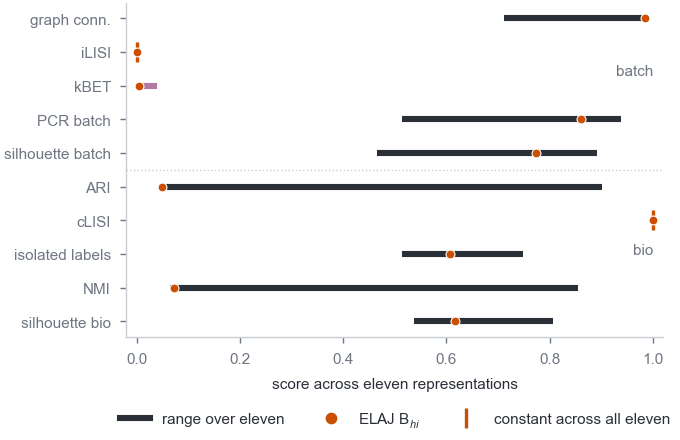
\includegraphics[width=.7\textwidth]{figures/scib_metric_range.png}
\caption[Range of each scIB metric]{\textbf{The range each metric spans
across eleven representations}, with \elaj\,B\textsubscript{hi}'s own score
marked. Two metrics have no range at all; kBET's is 0.04.}
\label{sfig:scib-range}
\end{figure}

\subsection{Where it discriminates, it ranks on something else}

Across the eleven representations no scIB metric tracks either axis the
paper reports (Table~\ref{stab:scib-corr}, Supplementary
Fig.~\ref{sfig:scib-corr}). The largest association in either direction is
graph connectivity against donor recovery at Spearman $\rho = -0.600$,
$P = 0.051$; every other coefficient has $|\rho| \leq 0.34$. The reason is
where the batch half looks. Each of its five metrics is defined against the
declared batch, which is study. The confound in this corpus sits one level
below: 254 donors nested inside eleven studies, each donor biopsied once, so
that menstrual phase, disease status and severity are constant within a
donor. A metric that asks whether studies mix is silent on whether donors
do, and donors are the level at which the biology is collinear with the
batch. Donor recovery is the quantity that sees this, and the cross-donor
estimator discards the same-donor part before it scores anything. A
representation can score well on every batch metric here while placing each
person in their own territory, and the one that does so most, by donor
recovery, is not the one scIB ranks last.

\begin{table}[t]
\centering
\caption[scIB metrics against the paper's axes]{\textbf{Each scIB metric
against donor recovery and against cross-donor cycle agreement.} Spearman
rank correlations across the eleven representations; the two constant
metrics have no rank order to correlate.}
\label{stab:scib-corr}
\small
% GENERATED by figures/scripts/supp_figures.py. Do not edit by hand.
\begin{tabular}{@{}llrrrr@{}}
\toprule
metric & half & $\rho$ donor recovery & $P$ & $\rho$ cycle & $P$ \\
\midrule
graph conn. & batch & $-$0.600 & 0.051 & 0.100 & 0.770 \\
iLISI & batch & -- & -- & -- & -- \\
kBET & batch & $-$0.265 & 0.431 & $-$0.192 & 0.572 \\
PCR batch & batch & $-$0.336 & 0.312 & 0.091 & 0.790 \\
silhouette batch & batch & $-$0.164 & 0.631 & $-$0.082 & 0.811 \\
\midrule
ARI & bio & 0.245 & 0.467 & $-$0.136 & 0.689 \\
cLISI & bio & -- & -- & -- & -- \\
isolated labels & bio & 0.218 & 0.519 & $-$0.073 & 0.832 \\
NMI & bio & 0.091 & 0.790 & $-$0.155 & 0.650 \\
silhouette bio & bio & 0.228 & 0.501 & 0.118 & 0.729 \\
\bottomrule
\end{tabular}

\end{table}

\begin{figure}[t]
\centering
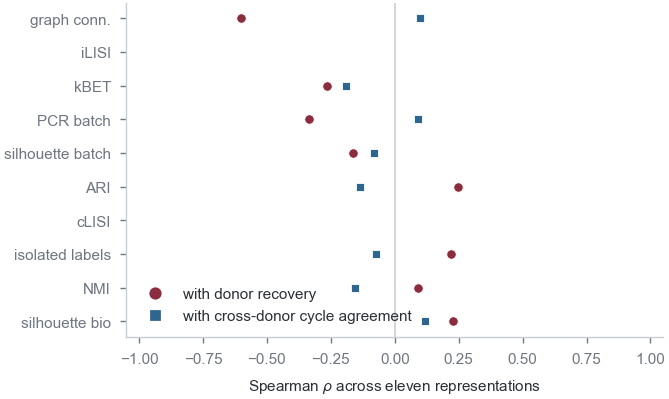
\includegraphics[width=.7\textwidth]{figures/scib_vs_donor_and_cycle.png}
\caption[scIB metrics against donor recovery and cycle]{\textbf{Table~\ref{stab:scib-corr}
drawn.} No metric in either half reaches $|\rho| = 0.65$ with either axis.}
\label{sfig:scib-corr}
\end{figure}

\subsection{The biological half rewards clustering, and clustering is not what this latent does}

ARI and NMI run Leiden clustering over a sweep of resolutions and report the
best agreement between clusters and the label. On them \elaj\,B\textsubscript{hi}
is last of eleven, at 0.0498 and 0.0724, and SCimilarity, which is
pretrained with supervision on cell type, is first at 0.9010 and 0.8555.
The same latent scores 0.9854 on graph connectivity, second of eleven and
0.0001 below scVI, 0.9820 on cross-donor cell family and 0.9864 on
$k$NN cell family. Those are two pictures of one representation. Each family
occupies a connected region and a cell's neighbours are its own family, but
the region does not break into discrete clusters at any resolution the
sweep visits, because inside each family the latent is organised along the
menstrual cycle (Supplementary Note~\ref{note:frontier},
Fig.~\ref{sfig:umap-base-phase}). A clustering metric is built to reward a
latent that falls into pieces coinciding with the label; a latent that is
continuous within the label scores low on it by construction, and the
cycle it is continuous along is the biology the paper is about.

The two \elaj{} arms make the mechanism visible
(Supplementary Fig.~\ref{sfig:scib-two-arms}). \elaj\,B\textsubscript{lo},
trained with the thirty-fold stronger prior, scores 0.1708 and 0.3364 on
ARI and NMI against B\textsubscript{hi}'s 0.0498 and 0.0724, while scoring
lower on cross-donor cell family, 0.9565 against 0.9820, and on the cycle,
0.6033 against 0.7346. Across the one coefficient that separates the two
arms, the clustering metrics and the neighbourhood metrics move in opposite
directions. On the remaining two biological metrics, isolated labels and
the biological silhouette, both arms sit inside the field's range, 0.5145
to 0.7483 and 0.5363 to 0.8060.

\begin{figure}[t]
\centering
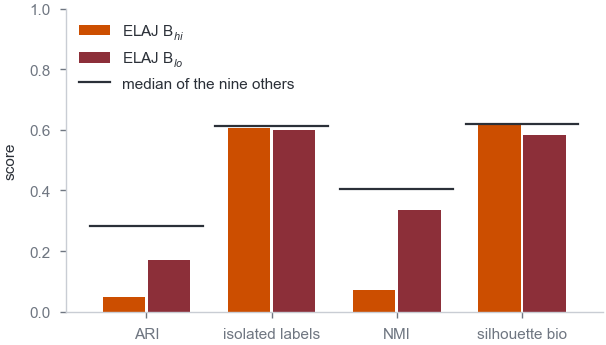
\includegraphics[width=.7\textwidth]{figures/scib_bio_half_two_arms.png}
\caption[The bio half on the two reported arms]{\textbf{The biological
half of the scorecard on the two reported arms}, against the median of the
nine other representations. The stronger prior raises the two clustering
metrics and lowers the neighbourhood ones.}
\label{sfig:scib-two-arms}
\end{figure}

\subsection{What this means for the paper}

Naming the axes: on scIB's clustering metrics \elaj{} is last of eleven; on
its connectivity metric it is second; on the paper's own instruments it is
first on the cycle and lowest on donor recovery. None of these is wrong.
They measure different things, and the one sentence the Discussion spends
on scIB, that its biological half is saturated on this corpus, rests on
Table~\ref{stab:scib-disc}: two constants, one near-constant, and a
biological half whose target label every method recovers. On an atlas built
from many datasets with cell type as the quantity to conserve, the same
battery discriminates as it was designed to. The corpus here is the case it
was not designed for, which is what made a corpus-specific instrument a
necessity rather than a preference.
